\documentclass[aspectratio=169,10pt]{beamer}
\usepackage[provide=*,spanish]{babel}
\usepackage{fontspec}
\setsansfont{Latin Modern Sans}
\usepackage{booktabs,tabularx,tikz,graphicx}
\usetikzlibrary{arrows.meta,positioning}
\newcolumntype{Y}{>{\raggedright\arraybackslash}X}
\definecolor{navy}{HTML}{14324C}
\definecolor{teal}{HTML}{008A89}
\definecolor{pale}{HTML}{EAF5F4}
\definecolor{softgold}{HTML}{FFF3DC}
\setbeamercolor{structure}{fg=teal}
\setbeamercolor{frametitle}{fg=white,bg=navy}
\setbeamercolor{block title}{fg=white,bg=navy}
\setbeamercolor{block body}{fg=navy,bg=pale}
\setbeamertemplate{navigation symbols}{}
\setbeamertemplate{footline}{\hfill\insertframenumber\hspace{4mm}\vspace{2mm}}
\title{Sistema adaptativo de detección de fraude}
\subtitle{IEEE-CIS Fraud Detection · Proyecto 1}
\author{Equipo: \underline{\hspace{6cm}}}
\institute{UTEC · Planificación y Toma de Decisiones en IA}
\date{2026-1}
\begin{document}

\begin{frame}
\titlepage
\vspace{-4mm}
\begin{center}\footnotesize Defensa diseñada para 15--20 minutos: problema, EDA, modelos, decisión, despliegue y adaptación.\end{center}
\end{frame}

\begin{frame}{Ruta de la presentación}\small
\begin{tabularx}{\linewidth}{@{}p{.18\linewidth}X p{.20\linewidth}@{}}\toprule
Tiempo & Contenido & Evidencia\\\midrule
2 min & Problema, objetivos y restricciones & Consigna y rúbrica\\
4 min & EDA y decisiones de preparación & EDA propio y referencia externa\\
5 min & Modelado V01--V07 y selección & Métricas de Kaggle\\
4 min & Política, incertidumbre y despliegue & V05, V06 y taller GCP\\
3 min & Drift, adaptación, límites y cierre & Protocolo de ciclo de vida\\\bottomrule
\end{tabularx}
\vfill
\begin{block}{Idea guía}
La entrega defiende un sistema de decisión adaptativo. El modelo predice riesgo, la política decide una acción y el monitoreo define cuándo ajustar el sistema.
\end{block}
\end{frame}

\begin{frame}{Problema y alcance}\small
\begin{columns}[T]
\column{.52\linewidth}
\begin{itemize}
\item El caso de uso es fraude financiero en transacciones electrónicas.
\item Cada transacción futura debe recibir una acción: aprobar, revisar o escalar.
\item La etiqueta positiva es minoritaria: 3.50\% de fraude en entrenamiento.
\end{itemize}
\column{.44\linewidth}
\begin{block}{Alcance responsable}
El sistema automatiza casos de bajo riesgo. Los casos ambiguos o de alto riesgo mantienen revisión humana y trazabilidad de la decisión.
\end{block}
\end{columns}
\vfill
\footnotesize La consigna pide un sistema inteligente adaptativo. Por eso la solución cubre predicción, decisión, acción, monitoreo y actualización.
\end{frame}

\begin{frame}{Objetivos, restricciones y métricas}\small
\begin{tabularx}{\linewidth}{@{}p{.24\linewidth}XX@{}}\toprule
Decisión de diseño & Por qué importa & Métrica usada\\\midrule
Priorizar fraude minoritario & Accuracy puede ser engañosa con 3.50\% de positivos & PR-AUC y recall\\
Separar pasado y futuro & Un split aleatorio sobreestima el rendimiento operativo & Validación temporal\\
Limitar revisión humana & El equipo operativo no puede revisar todo & Tasa de revisión y costo\\
Controlar incertidumbre & Un score alto no equivale a probabilidad calibrada & Brier y calibración\\
Adaptarse al cambio & Los patrones de fraude cambian por ventana & KS, PSI y métricas semanales\\\bottomrule
\end{tabularx}
\vfill
\begin{block}{Criterio}
PR-AUC es la métrica principal porque evalúa directamente el ranking de la clase minoritaria. ROC-AUC se reporta como complemento.
\end{block}
\end{frame}

\begin{frame}{EDA temporal}\small
\begin{columns}[T]
\column{.48\linewidth}
\begin{block}{Hallazgos del equipo}
590\,540 transacciones etiquetadas, 506\,691 sin etiqueta, tasa global de fraude de 3.499\% y tasa semanal entre 1.85\% y 5.06\%.
\end{block}
\begin{itemize}
\item 74 variables superan 80\% de faltantes.
\item Train y test se separan con adversarial ROC-AUC 1.000.
\end{itemize}
\column{.48\linewidth}
\begin{block}{Lectura}
La evidencia muestra cambio temporal observable. No prueba sola que cambie $P(Y\mid X)$, pero sí obliga a validar con orden cronológico y monitorear ventanas futuras.
\end{block}
\end{columns}
\end{frame}

\begin{frame}{EDA de referencia y ajustes incorporados}\small
\begin{tabularx}{\linewidth}{@{}>{\raggedright\arraybackslash}p{.30\linewidth}YY@{}}\toprule
Aporte revisado & Riesgo si se ignora & Decisión tomada\\\midrule
Faltantes de identidad & Tratar ausencia como ruido aleatorio & Mantener señal de identidad y reportar segmento UID\\
Faltantes por bloques V & Eliminar variables útiles por missingness alto & Auditar por grupos y no podar de forma automática\\
Monto con cola pesada & Borrar transacciones raras que pueden ser fraude & No eliminar outliers de monto\\
Montos con más de dos decimales & Perder una señal transaccional sencilla & Agregar indicador multi-decimal en V07\\
MLP como comparación & Asumir que boosting basta sin contrastar & Ejecutar V07 con MLP ponderado\\\bottomrule
\end{tabularx}
\vfill
\footnotesize El notebook externo se usó como insumo metodológico, no como fuente de métricas finales, porque usa otro split y otra política de costos.
\end{frame}

\begin{frame}{Preparación temporal}\small
\begin{center}
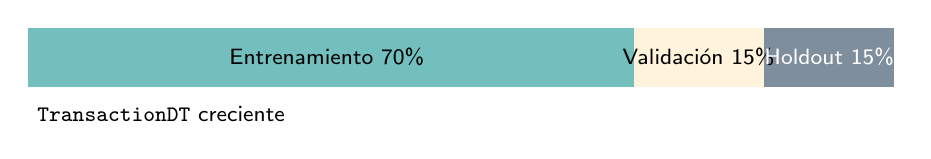
\begin{tikzpicture}[font=\sffamily\footnotesize,x=1cm,y=1cm]
\fill[navy!12] (0,0) rectangle (11,.75);
\fill[teal!55] (0,0) rectangle (7.7,.75);
\fill[softgold] (7.7,0) rectangle (9.35,.75);
\fill[navy!55] (9.35,0) rectangle (11,.75);
\node at (3.8,.38){Entrenamiento 70\%};
\node at (8.52,.38){Validación 15\%};
\node[text=white] at (10.18,.38){Holdout 15\%};
\node[anchor=west] at (0,-.35){\texttt{TransactionDT} creciente};
\end{tikzpicture}
\end{center}
\begin{itemize}
\item El preprocesamiento se ajusta con pasado y se aplica a validación y holdout.
\item \texttt{TransactionDT}, día y semana se excluyen como predictores para evitar posición temporal absoluta.
\item Las agregaciones UID sólo se aceptan si usan eventos previos a la transacción.
\end{itemize}
\begin{block}{Justificación}
El sistema operaría sobre transacciones futuras. La evaluación debe imitar esa condición.
\end{block}
\end{frame}

\begin{frame}{Diseño experimental V01--V07}\small
\begin{tabularx}{\linewidth}{@{}p{.12\linewidth}X X@{}}\toprule
Versión & Pregunta que responde & Decisión\\\midrule
V01 & ¿Qué tan fuerte es un LightGBM temporal con features auditables? & Modelo base\\
V01b & ¿Conviene usar todas las features sin filtro? & No, empeora holdout\\
V02 & ¿La memoria de UID ayuda? & Ayuda sólo en UID conocido\\
V03 & ¿Qué variables conservar o vigilar? & Usar como auditoría\\
V04 & ¿Otro boosting supera al baseline? & No supera V01\\
V05 & ¿Cómo convertir score en acción? & Política inicial\\
V06 & ¿Qué tan calibrado y robusto es el score? & Calibrar si se comunica probabilidad\\
V07 & ¿Un MLP o baseline lineal mejora? & No reemplaza LightGBM\\\bottomrule
\end{tabularx}
\end{frame}

\begin{frame}{Resultados del modelo base}\small
\begin{center}
\begin{tabular}{@{}lrrr@{}}\toprule
Bloque & Fraude & PR-AUC & ROC-AUC\\\midrule
Validación global & 3.43\% & 0.5954 & 0.9257\\
Holdout global & 3.48\% & 0.5436 & 0.9051\\
Holdout UID conocido & 1.93\% & 0.5159 & 0.9020\\
Holdout UID desconocido & 4.73\% & 0.5632 & 0.8933\\\bottomrule
\end{tabular}
\end{center}
\begin{block}{Lectura}
La caída de PR-AUC entre validación y holdout confirma que el rendimiento se degrada con el tiempo. Aun así, V01 conserva el mejor balance entre desempeño y generalización.
\end{block}
\end{frame}

\begin{frame}{Comparaciones que no reemplazaron V01}\small
\begin{tabularx}{\linewidth}{@{}p{.22\linewidth}p{.24\linewidth}X@{}}\toprule
Experimento & Resultado & Motivo de descarte\\\midrule
V01b con todas las features & Holdout PR-AUC 0.5303 & Más variables no implicaron mejor generalización temporal\\
V02 con UID histórico & Global 0.5442, UID unknown 0.5315 & Riesgo para clientes no vistos\\
V04 con features auditadas & Mejor candidato 0.5131 & Podar agresivamente eliminó señal útil\\
V07 MLP ponderado & Holdout PR-AUC 0.2218 & No aprovecha tan bien faltantes e interacciones tabulares\\
V07 SGD logística & Holdout PR-AUC 0.1638 & Baseline lineal insuficiente para la estructura del problema\\\bottomrule
\end{tabularx}
\vfill
\footnotesize La decisión no se basó en popularidad de modelos, sino en evidencia temporal comparable.
\end{frame}

\begin{frame}{Política V05}\small
\begin{columns}[T]
\column{.48\linewidth}
\begin{block}{Reglas}
$s<0.459783$: aprobar.\\
$0.459783\leq s<0.779122$: revisión.\\
$s\geq0.779122$: escalar.
\end{block}
\begin{itemize}
\item Fraude aprobado: costo 100.
\item Legítima escalada: costo 10.
\item Revisión manual: costo 2.
\end{itemize}
\column{.48\linewidth}
\begin{block}{Holdout}
Costo por transacción 1.3680.\\
Fraude detectado 66.17\%.\\
Revisión 5.10\%.\\
Escalamiento 2.48\%.
\end{block}
La tasa de revisión supera levemente 5\%, así que producción requiere cupo estricto por percentil o cola operativa.
\end{columns}
\end{frame}

\begin{frame}{Incertidumbre y calibración V06}\small
\begin{columns}[T]
\column{.48\linewidth}
\begin{block}{Problema}
El score bruto rankea transacciones, pero no debe presentarse como probabilidad directa.
\end{block}
\begin{itemize}
\item Score bruto medio en holdout: 14.30\%.
\item Tasa real de fraude: 3.48\%.
\end{itemize}
\column{.48\linewidth}
\begin{block}{Solución evaluada}
Calibración isotónica entrenada con pasado.\\
Brier: 0.0479 a 0.0219.\\
Media calibrada: 3.55\%.
\end{block}
Uso recomendado: score bruto para ranking, score calibrado para comunicar probabilidad.
\end{columns}
\end{frame}

\begin{frame}{Arquitectura del sistema}\small
\begin{center}
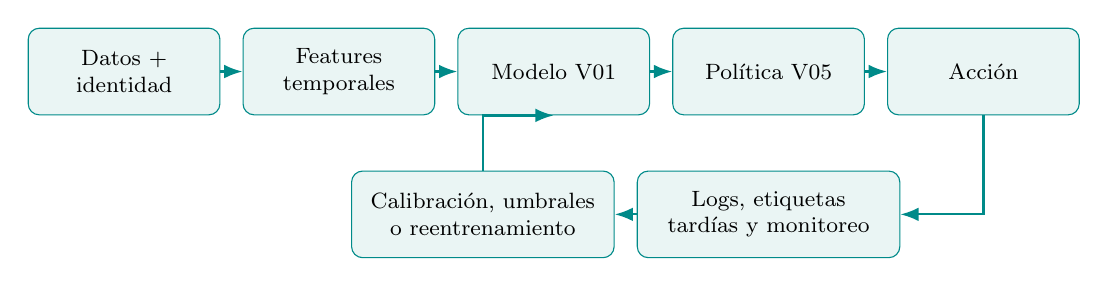
\begin{tikzpicture}[node distance=2.8mm,>=Latex,font=\footnotesize,
box/.style={draw=teal,rounded corners,fill=pale,align=center,text width=22mm,minimum height=11mm}]
\node[box](a){Datos + identidad};
\node[box,right=of a](b){Features temporales};
\node[box,right=of b](c){Modelo V01};
\node[box,right=of c](d){Política V05};
\node[box,right=of d](e){Acción};
\node[box,below=7mm of d,text width=31mm](f){Logs, etiquetas tardías y monitoreo};
\node[box,left=of f,text width=31mm](g){Calibración, umbrales o reentrenamiento};
\draw[->,thick,teal](a)--(b);
\draw[->,thick,teal](b)--(c);
\draw[->,thick,teal](c)--(d);
\draw[->,thick,teal](d)--(e);
\draw[->,thick,teal](e.south)|-(f.east);
\draw[->,thick,teal](f)--(g);
\draw[->,thick,teal](g.north)|-(c.south);
\end{tikzpicture}
\end{center}
\begin{block}{Nivel de autonomía}
Aprobación automática para bajo riesgo. Revisión humana para incertidumbre. Escalamiento con control y registro para alto riesgo.
\end{block}
\end{frame}

\begin{frame}{Despliegue propuesto en GCP}\small
\begin{tabularx}{\linewidth}{@{}p{.24\linewidth}X X@{}}\toprule
Componente & Función & Evidencia o control\\\midrule
FastAPI & Exponer \texttt{POST /predict} & Entrada, score, decisión y versión\\
Docker & Empaquetar código y dependencias & Misma imagen para prueba y producción\\
Artifact Registry & Versionar imágenes & Trazabilidad de releases\\
Cloud Build & Construir desde GitHub & Automatizar pipeline de despliegue\\
Cloud Run & Servir contenedor HTTP & Escalado administrado y logs integrados\\
Monitoring & Vigilar latencia, errores y drift & Alertas operativas y técnicas\\\bottomrule
\end{tabularx}
\vfill
\footnotesize El despliegue queda como diseño técnico basado en el taller GCP. Antes de operar faltan pruebas de carga, integración y seguridad.
\end{frame}

\begin{frame}{Drift y adaptación}\small
\begin{tabularx}{\linewidth}{@{}p{.25\linewidth}XX@{}}\toprule
Señal & Sin etiquetas & Con etiquetas tardías\\\midrule
Features & KS, PSI, missingness, percentiles & Relación con errores reales\\
Scores & Distribución del score y tasas sobre umbral & PR-AUC, Brier y recall\\
Operación & Revisión, escalamiento y latencia & Costo y fraude capturado\\
Segmentos & UID conocido y desconocido & Brechas de desempeño por segmento\\\bottomrule
\end{tabularx}
\vspace{3mm}
\begin{block}{Adaptación propuesta}
Comparar entrenamiento histórico frente a ventanas móviles de 4, 8 y 12 semanas. Promover una versión sólo si mejora en bloque futuro y no empeora UID desconocido.
\end{block}
\end{frame}

\begin{frame}{Mapa de rúbrica}\small
\begin{tabularx}{\linewidth}{@{}p{.31\linewidth}X@{}}\toprule
Criterio del curso & Evidencia en la entrega\\\midrule
Problema, objetivos y métricas & Caso fraude, restricciones, PR-AUC, costo, revisión y calibración\\
Análisis y preparación & EDA temporal, faltantes, UID, split 70/15/15 y control de leakage\\
Modelado y evaluación & V01--V07, comparación temporal, segmentación y holdout futuro\\
Sistema adaptativo & Arquitectura, acción, incertidumbre, drift y reentrenamiento\\
Producto entregado & Código Kaggle, GitHub, informes, diagramas, PDFs e infografía\\
Presentación & Guion de 15--20 minutos con defensa de decisiones\\\bottomrule
\end{tabularx}
\end{frame}

\begin{frame}{Limitaciones y riesgos}\small
\begin{tabularx}{\linewidth}{@{}p{.28\linewidth}X@{}}\toprule
Límite & Cómo se controla\\\midrule
Costos normalizados & Repetir sensibilidad cuando existan costos reales\\
Dataset anonimizado & Evitar causalidad fuerte sobre variables sin significado de negocio\\
Revisión 5.10\% & Aplicar cupo operativo estricto antes de producción\\
Equidad demográfica no observable & Usar proxies operativos disponibles y reportar la limitación\\
Drift futuro desconocido & Monitoreo por ventanas y validación antes de promover modelos\\\bottomrule
\end{tabularx}
\vfill
\begin{block}{Riesgo académico restante}
Si la lectura de la rúbrica exige dos modelos tradicionales estrictos, conviene agregar un Random Forest o HistGradientBoosting simple. No cambiaría la recomendación, pero cerraría el requisito formal.
\end{block}
\end{frame}

\begin{frame}{Conclusión}\small
\begin{block}{Decisión final}
Mantener V01 como modelo base, usar V05 como política inicial y usar V06 como soporte de calibración y robustez. V07 queda como benchmark adicional.
\end{block}
\begin{itemize}
\item V01 generaliza mejor en holdout temporal que las alternativas probadas.
\item V05 convierte el ranking en decisiones con costo y capacidad explícitos.
\item V06 evita comunicar scores brutos como probabilidades.
\item El monitoreo convierte el clasificador en un sistema adaptativo.
\end{itemize}
\vfill
\footnotesize La defensa central es conservadora: se elige la alternativa más estable y trazable, no la más compleja.
\end{frame}

\begin{frame}{Infografía del ciclo completo}
\centering
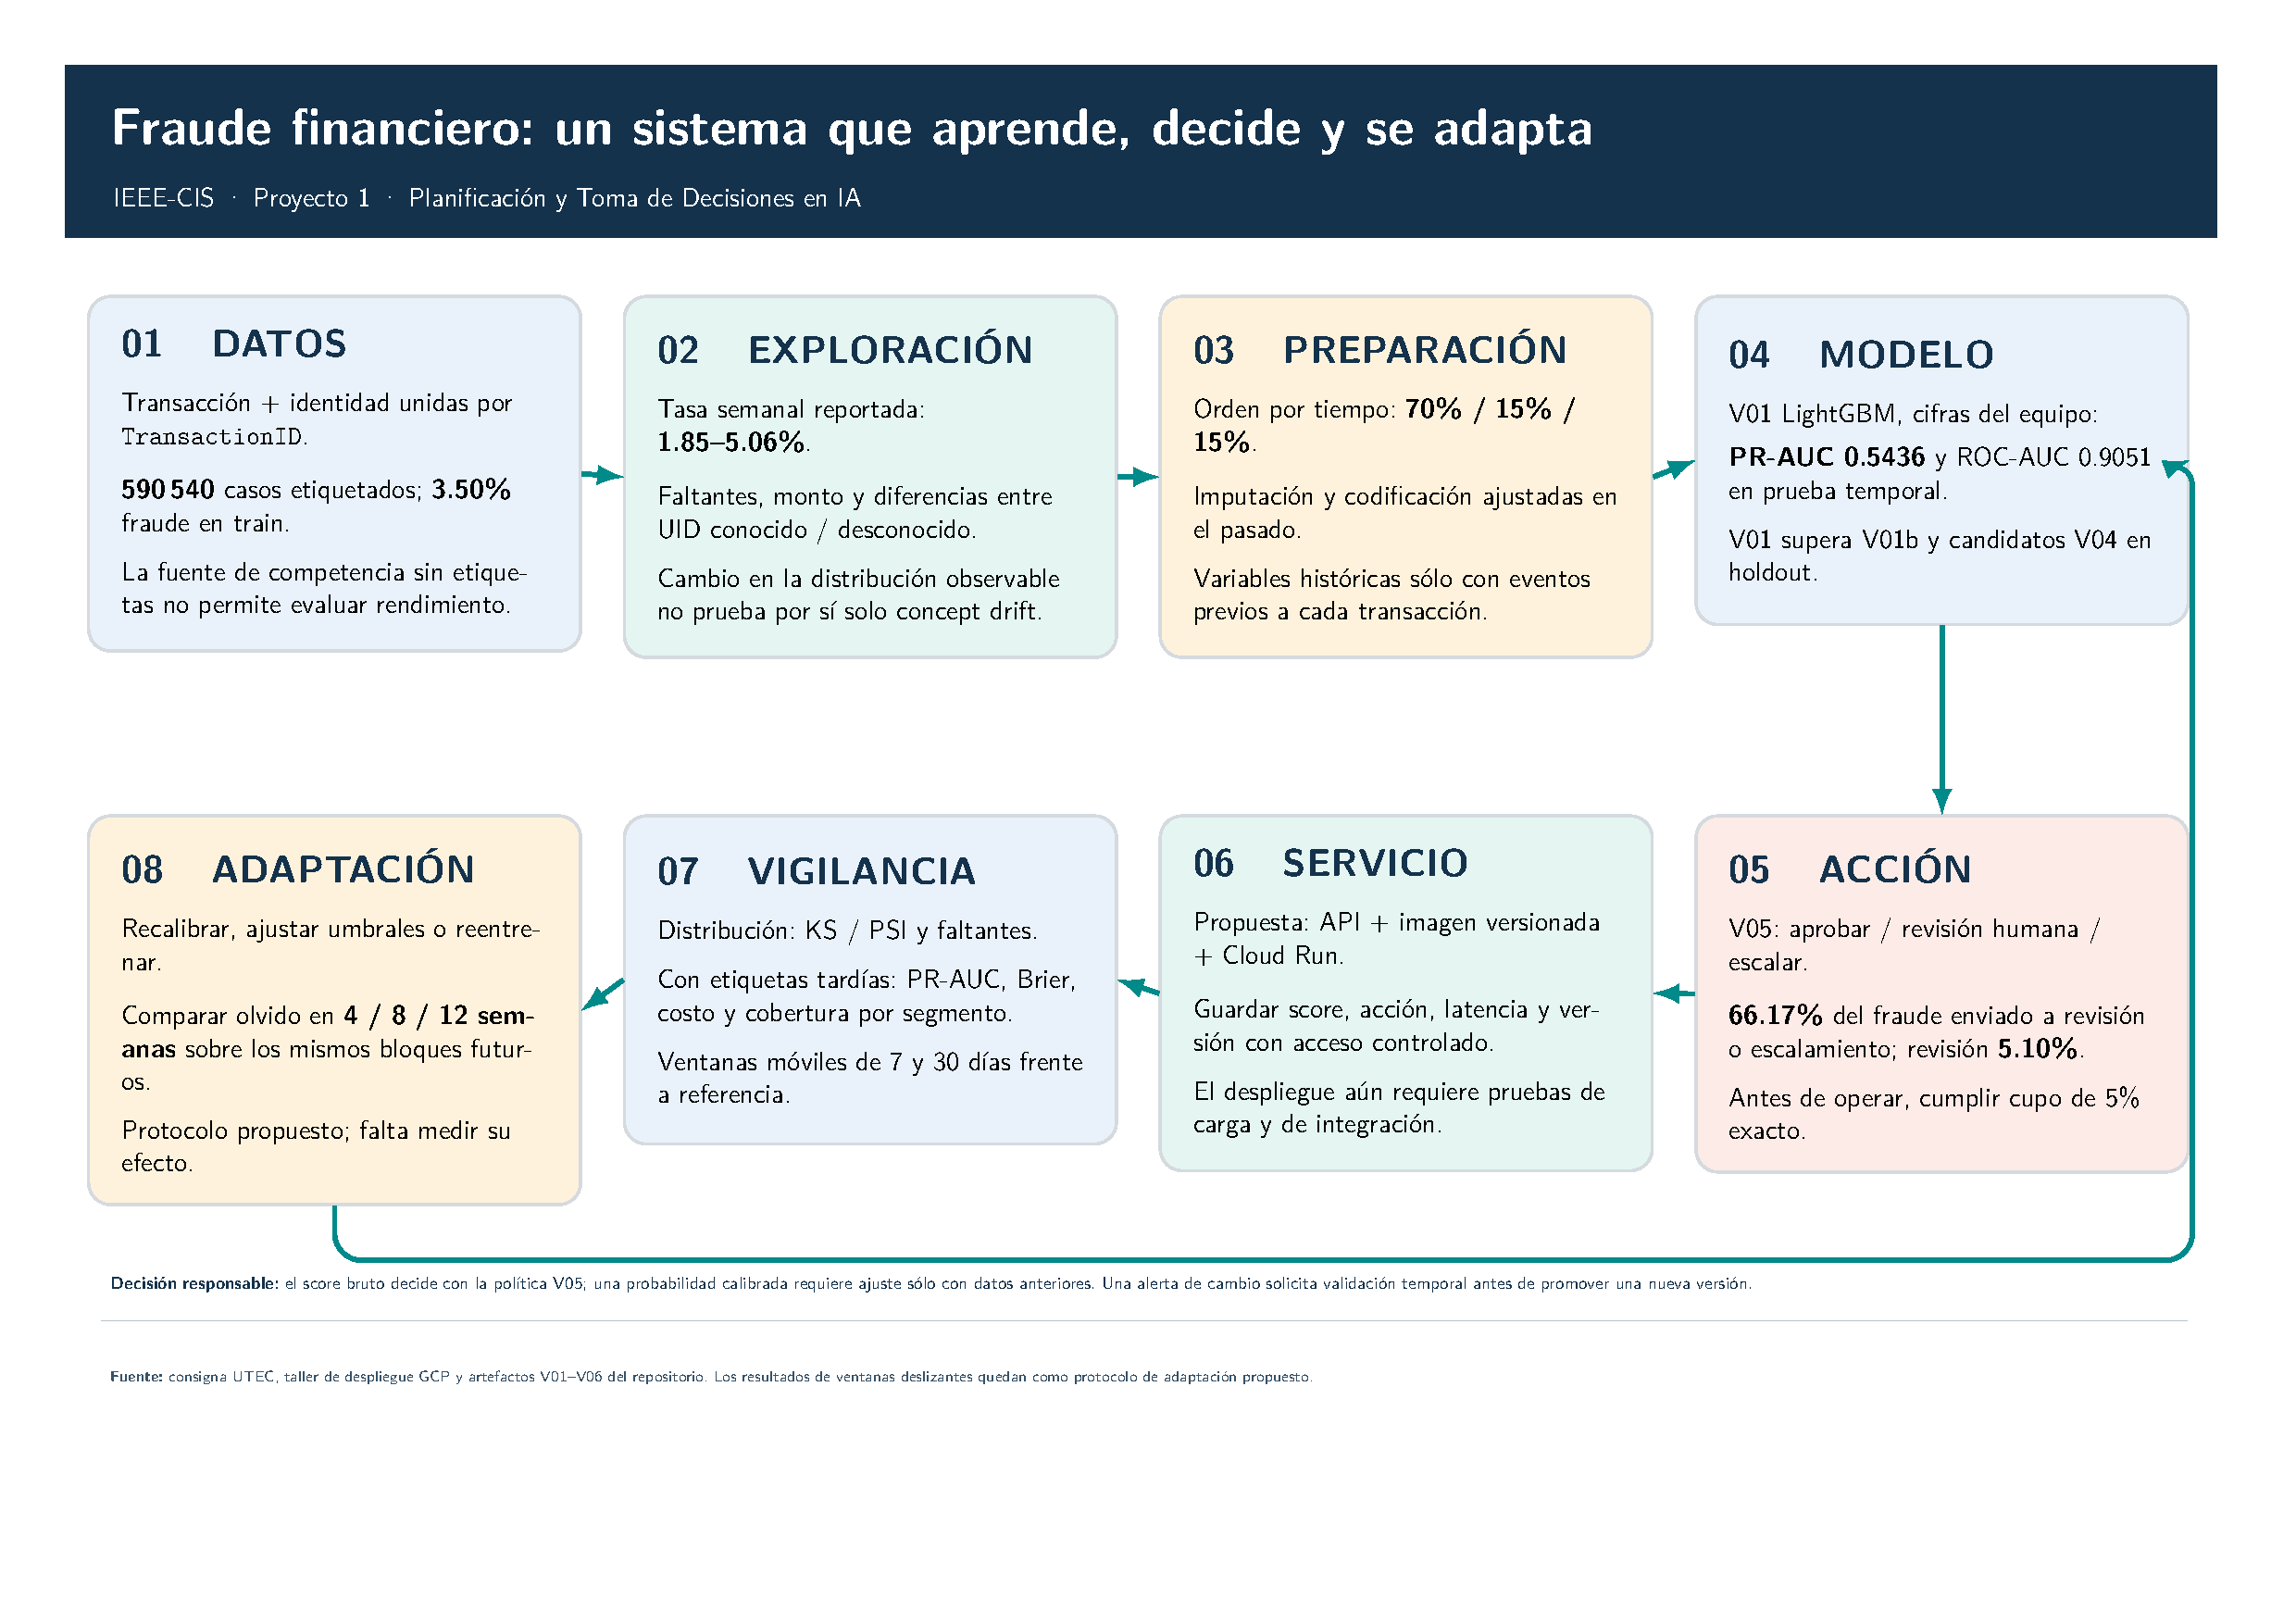
\includegraphics[width=\textwidth,height=.84\textheight,keepaspectratio]{infografia.pdf}
\end{frame}

\end{document}
